\documentclass[aspectratio=169,11pt]{beamer}

% ── Theme & Colors ──────────────────────────────────────────────────
\usetheme{metropolis}
\usepackage{appendixnumberbeamer}
\definecolor{strand}{RGB}{31,119,180}   % blue
\definecolor{coil}{RGB}{148,103,189}    % purple
\definecolor{helix}{RGB}{214,39,40}     % red
\definecolor{offset}{RGB}{44,160,44}    % green
\definecolor{outlier}{RGB}{180,180,180} % grey

% ── Packages ────────────────────────────────────────────────────────
\usepackage{pgfplots}
\pgfplotsset{compat=1.18}
\usepackage{booktabs}
\usepackage{multirow}
\usepackage{amsmath}
\usepackage{tikz}
\usetikzlibrary{arrows.meta,positioning,decorations.pathreplacing,calc}

% ── Footer: slide N/total ───────────────────────────────────────────
\setbeamertemplate{frame numbering}{\insertframenumber/\inserttotalframenumber}

% ── Title ───────────────────────────────────────────────────────────
\title{LACS --- Linear Analysis of Chemical Shifts}
\subtitle{Detecting \& Correcting NMR Referencing Errors}
\date{22 April 2026}
\author{Tobias Senoner}
\institute{TriZOD Project Meeting}

\begin{document}

\maketitle

% ═══════════════════════════════════════════════════════════════════
% SLIDE: The Problem
% ═══════════════════════════════════════════════════════════════════
\begin{frame}{The Problem: Referencing Errors}

\begin{columns}[T]
\begin{column}{0.55\textwidth}
Every NMR chemical shift is measured \textbf{relative to a reference standard}
(e.g.\ DSS for ${}^{13}$C).

\smallskip
If the reference is wrong by a constant $k$:
\[
  \delta_{\text{obs}} = \delta_{\text{true}} + k
  \qquad \forall\;\text{atoms of that nucleus type}
\]

\smallskip
\textbf{Prevalence in the BMRB:}
\begin{itemize}\setlength\itemsep{1pt}
  \item $\sim$20\% of ${}^{13}$C entries mis-referenced
  \item $\sim$35\% of ${}^{15}$N entries mis-referenced
\end{itemize}

\smallskip
\alert{Undetected offsets bias every downstream analysis.}
\end{column}

\begin{column}{0.40\textwidth}
\centering
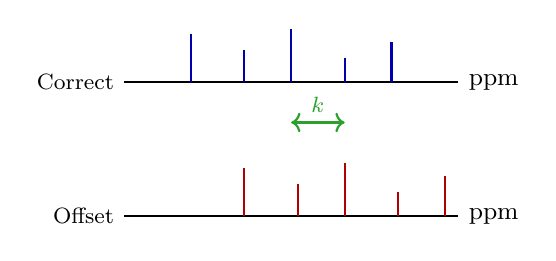
\begin{tikzpicture}[scale=0.85]
  % Correct spectrum
  \draw[thick] (0,3.5) -- (5,3.5) node[right]{\small ppm};
  \node[left] at (0,3.5) {\footnotesize Correct};
  \foreach \x/\h in {1.0/1.8, 1.8/1.2, 2.5/2.0, 3.3/0.9, 4.0/1.5} {
    \draw[blue!70!black,thick] (\x,3.5) -- (\x,3.5+\h*0.4);
  }
  % Offset spectrum
  \draw[thick] (0,1.5) -- (5,1.5) node[right]{\small ppm};
  \node[left] at (0,1.5) {\footnotesize Offset};
  \foreach \x/\h in {1.0/1.8, 1.8/1.2, 2.5/2.0, 3.3/0.9, 4.0/1.5} {
    \pgfmathsetmacro{\xshift}{\x+0.8}
    \draw[red!70!black,thick] (\xshift,1.5) -- (\xshift,1.5+\h*0.4);
  }
  % Arrow showing offset k
  \draw[<->,thick,offset] (2.5,2.9) -- node[above]{\footnotesize $k$} (3.3,2.9);
\end{tikzpicture}
\end{column}
\end{columns}

\smallskip
\footnotesize
Wang et al.\ (2005) \textit{J Biomol NMR} 32:13--22;\;
Wang \& Markley (2009) \textit{J Biomol NMR} 44:95--99
\end{frame}

% ═══════════════════════════════════════════════════════════════════
% SLIDE: The Core Insight
% ═══════════════════════════════════════════════════════════════════
\begin{frame}{The Core Insight: Offset Cancellation}

The \textbf{difference} of two ${}^{13}$C atoms is immune to the offset:
\[
\boxed{
(\text{CA}_\text{obs} - \text{CB}_\text{obs})
= (\text{CA}_\text{true} + k) - (\text{CB}_\text{true} + k)
= \text{CA}_\text{true} - \text{CB}_\text{true}
}
\]

\smallskip
\begin{columns}[T]
\begin{column}{0.50\textwidth}
\textbf{LACS strategy:}
\begin{enumerate}\setlength\itemsep{1pt}
  \item \textbf{X-axis}: secondary shift of the CA$-$CB \emph{difference} (offset-free)
  \item \textbf{Y-axis}: secondary shift of CA (retains offset $k$)
  \item Non-zero \textbf{Y-intercept} $= k$
\end{enumerate}
\end{column}
\begin{column}{0.48\textwidth}
\centering
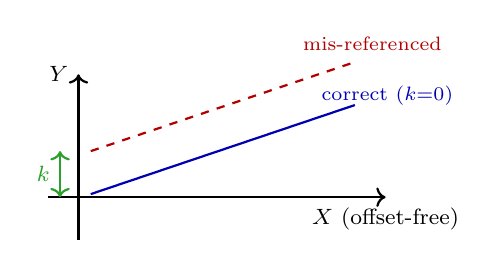
\begin{tikzpicture}[scale=0.78]
  \draw[->,thick] (-0.5,0) -- (5,0) node[below] {\footnotesize$X$ (offset-free)};
  \draw[->,thick] (0,-0.7) -- (0,2) node[left] {\footnotesize$Y$};
  \draw[blue!70!black, thick] (0.2,0.05) -- (4.5,1.5);
  \node[blue!70!black,right] at (3.8,1.65) {\scriptsize correct ($k{=}0$)};
  \draw[red!70!black, thick, dashed] (0.2,0.75) -- (4.5,2.2);
  \node[red!70!black,right] at (3.5,2.5) {\scriptsize mis-referenced};
  \draw[<->,thick,offset] (-0.3,0) -- node[left]{\footnotesize $k$} (-0.3,0.75);
\end{tikzpicture}
\end{column}
\end{columns}
\end{frame}

% ═══════════════════════════════════════════════════════════════════
% SLIDE: Algorithm Overview
% ═══════════════════════════════════════════════════════════════════
\begin{frame}{LACS Algorithm Overview (${}^{13}$C / ${}^{1}$H$_\alpha$)}

\begin{center}
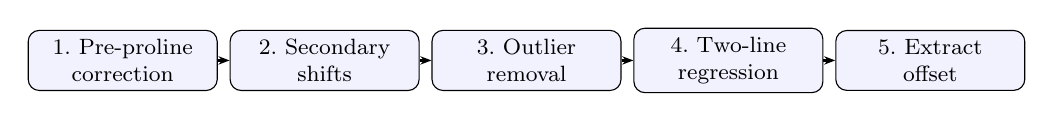
\begin{tikzpicture}[
  box/.style={draw, rounded corners, fill=blue!5, minimum height=0.7cm, minimum width=2.4cm, align=center, font=\footnotesize},
  arr/.style={-{Stealth[length=4pt]}, thick},
  node distance=0.15cm
]
  \node[box] (s1) {1.\ Pre-proline\\correction};
  \node[box, right=of s1] (s2) {2.\ Secondary\\shifts};
  \node[box, right=of s2] (s3) {3.\ Outlier\\removal};
  \node[box, right=of s3] (s4) {4.\ Two-line\\regression};
  \node[box, right=of s4] (s5) {5.\ Extract\\offset};

  \draw[arr] (s1) -- (s2);
  \draw[arr] (s2) -- (s3);
  \draw[arr] (s3) -- (s4);
  \draw[arr] (s4) -- (s5);
\end{tikzpicture}
\end{center}

\medskip

\begin{columns}[T]
\begin{column}{0.48\textwidth}
\textbf{Applies to:}
\begin{itemize}
  \item CA, CB, C$'$ (CO), H$_\alpha$ (HA)
  \item Excludes: Cys, Gly, Pro
  \item Requires $\geq 20$ valid residues
\end{itemize}
\end{column}
\begin{column}{0.48\textwidth}
\textbf{Reference tables:}
\begin{itemize}
  \item Random coil shifts (Wishart 1995)
  \item Pre-proline corrections (20 AA)
  \item Thresholds per atom type
\end{itemize}
\end{column}
\end{columns}
\end{frame}

% ═══════════════════════════════════════════════════════════════════
% SLIDE: Step 1 — Pre-proline correction
% ═══════════════════════════════════════════════════════════════════
\begin{frame}[shrink=8]{Step 1: Pre-Proline Correction}

Proline's cyclic side chain systematically perturbs shifts of the \textbf{preceding residue}.

\medskip
Before computing secondary shifts, add amino-acid-specific corrections to residue $i$ when residue $i{+}1$ is Pro:

\[
\delta^{\text{corr}}_{i} = \delta^{\text{obs}}_{i} + \Delta_{\text{pre-Pro}}(\text{AA}_i, \text{atom})
\]

\medskip
\begin{center}
\footnotesize
\begin{tabular}{lcccccc}
\toprule
AA & $\Delta$CA & $\Delta$CB & $\Delta$HA & $\Delta$CO & $\Delta$H & $\Delta$N \\
\midrule
Ala & +2.0 & +1.0 & $-$0.30 & +1.9 & +0.05 & $-$1.2 \\
Val & +2.4 & +0.3 & $-$0.32 & +1.4 & +0.01 & $-$1.3 \\
Leu & +2.0 & +0.7 & $-$0.34 & +1.9 & +0.02 & $-$0.8 \\
\ldots & \ldots & \ldots & \ldots & \ldots & \ldots & \ldots \\
\bottomrule
\end{tabular}
\end{center}

\medskip
\textbf{Purpose:} Remove this known systematic effect so it doesn't contaminate the offset estimate.
\end{frame}

% ═══════════════════════════════════════════════════════════════════
% SLIDE: Step 2 — Computing secondary shifts
% ═══════════════════════════════════════════════════════════════════
\begin{frame}{Step 2: Secondary Shifts --- X and Y Axes}

For each valid residue $i$ with amino acid type $a$:

\smallskip
\textbf{X-axis} (reference-independent):
\[
  X_i = \underbrace{(\text{CA}^{\text{obs}}_i - \text{CB}^{\text{obs}}_i)}_{\text{observed diff.}}
      - \underbrace{(\text{CA}^{\text{rc}}_a - \text{CB}^{\text{rc}}_a)}_{\text{random coil diff.}}
\]
Any ${}^{13}$C referencing error $k$ cancels: $(x{+}k){-}(y{+}k) = x{-}y$.

\smallskip
\textbf{Y-axis} (retains the offset):
\[
  Y_i = \text{target}^{\text{obs}}_i - \text{target}^{\text{rc}}_a
  \qquad \text{(target = CA, CB, CO, or HA)}
\]

\begin{exampleblock}{Worked Example: Val-15 in bmr10260}
\small
$\text{CA}_\text{obs} = 58.57$,\; $\text{CB}_\text{obs} = 34.15$,\;
$\text{CA}_\text{rc} = 62.2$,\; $\text{CB}_\text{rc} = 32.9$ \\[2pt]
$X = (58.57 - 34.15) - (62.2 - 32.9) = -4.88$ \\[1pt]
$Y_\text{CA} = 58.57 - 62.2 = -3.63$
\end{exampleblock}
\end{frame}

% ═══════════════════════════════════════════════════════════════════
% SLIDE: Step 3 — The V-shape
% ═══════════════════════════════════════════════════════════════════
\begin{frame}[shrink=8]{The V-Shape: Secondary Structure Creates Two Branches}

\begin{columns}[T]
\begin{column}{0.45\textwidth}
The CA$-$CB secondary shift correlates with secondary structure:

\bigskip
\begin{tabular}{ll}
\textcolor{helix}{\textbf{Helix}} & $X \gg 0$ \\
& (high CA, low CB) \\[4pt]
\textcolor{coil}{\textbf{Coil}} & $X \approx 0$ \\[4pt]
\textcolor{strand}{\textbf{Strand}} & $X \ll 0$ \\
& (low CA, high CB) \\
\end{tabular}

\bigskip
The Y-axis ($\Delta\delta$ of any single atom) has a \textbf{different slope} vs.\ X for helix vs.\ strand residues.

\medskip
$\Rightarrow$ \textbf{Two-line fit} to capture both branches.
\end{column}

\begin{column}{0.52\textwidth}
\centering
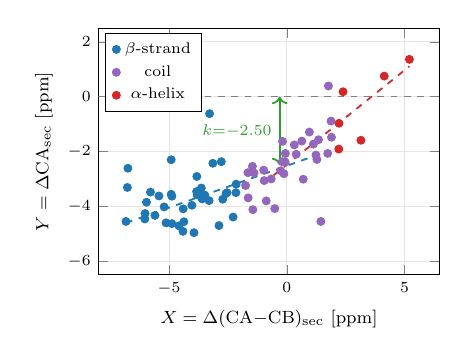
\begin{tikzpicture}[scale=0.8]
\begin{axis}[
  width=7cm, height=5.5cm,
  xlabel={$X = \Delta(\text{CA}{-}\text{CB})_\text{sec}$ [ppm]},
  ylabel={$Y = \Delta\text{CA}_\text{sec}$ [ppm]},
  xlabel style={font=\footnotesize},
  ylabel style={font=\footnotesize},
  tick label style={font=\scriptsize},
  xmin=-8, xmax=6.5,
  ymin=-6.5, ymax=2.5,
  grid=major,
  grid style={gray!20},
  legend style={at={(0.02,0.98)}, anchor=north west, font=\scriptsize},
]

% Strand points (blue)
\addplot[only marks, mark=*, mark size=1.8pt, strand] coordinates {
  (-6.02, -4.26) (-4.88, -3.63) (-3.82, -2.91) (-3.63, -3.33)
  (-2.72, -3.74) (-3.94, -4.96) (-5.96, -3.85) (-4.91, -3.56)
  (-6.03, -4.46) (-3.59, -3.72) (-5.21, -4.02) (-4.91, -2.30)
  (-2.15, -3.19) (-3.81, -3.58) (-2.54, -3.50) (-4.41, -4.91)
  (-6.83, -4.55) (-3.77, -3.55) (-2.58, -3.53) (-5.43, -3.62)
  (-4.40, -4.09) (-2.88, -4.70) (-3.60, -3.72) (-3.28, -0.62)
  (-2.78, -2.37) (-3.30, -3.79) (-6.75, -2.61) (-5.13, -4.60)
  (-5.79, -3.48) (-3.48, -3.59) (-4.88, -4.63) (-3.83, -3.46)
  (-5.60, -4.33) (-2.28, -4.39) (-3.14, -2.43) (-2.16, -3.50)
  (-4.58, -4.71) (-4.03, -3.96) (-6.77, -3.31) (-4.37, -4.56)
};
\addlegendentry{$\beta$-strand}

% Coil points (purple)
\addplot[only marks, mark=*, mark size=1.8pt, coil] coordinates {
  (-0.98, -2.68) (1.74, -2.07) (0.96, -1.29) (0.70, -3.01)
  (1.90, -1.48) (0.40, -2.10) (-0.96, -3.06) (1.77, 0.39)
  (1.35, -1.57) (-0.07, -2.38) (-0.87, -3.80) (1.24, -2.13)
  (1.13, -1.73) (-1.64, -3.69) (1.88, -0.89) (-0.26, -2.70)
  (-1.46, -2.54) (-0.18, -1.63) (1.45, -4.55) (-1.44, -4.12)
  (-0.12, -2.81) (-0.51, -4.08) (0.32, -1.76) (1.28, -2.29)
  (-1.75, -3.24) (-1.39, -2.78) (0.64, -1.62) (-0.66, -3.00)
  (-1.65, -2.77) (-0.06, -2.07) (-0.19, -2.37)
};
\addlegendentry{coil}

% Helix points (red)
\addplot[only marks, mark=*, mark size=1.8pt, helix] coordinates {
  (3.15, -1.59) (2.39, 0.18) (5.21, 1.36)
  (2.22, -0.97) (4.14, 0.75) (2.21, -1.91)
};
\addlegendentry{$\alpha$-helix}

% Strand-side regression line
\addplot[strand, thick, dashed, domain=-6.83:1.0] {-2.521 + 0.305*x};

% Helix-side regression line
\addplot[helix, thick, dashed, domain=-1.0:5.21] {-2.483 + 0.689*x};

% Zero line and offset annotation
\draw[thin,gray,dashed] (axis cs:-8,0) -- (axis cs:6.5,0);
\draw[<->,thick,offset] (axis cs:-0.3,-2.50) -- node[left,font=\scriptsize,offset]
  {$k{=}{-}2.50$} (axis cs:-0.3,0);

\end{axis}
\end{tikzpicture}
\end{column}
\end{columns}
\end{frame}

% ═══════════════════════════════════════════════════════════════════
% SLIDE: Step 3 — Outlier removal
% ═══════════════════════════════════════════════════════════════════
\begin{frame}[shrink=8]{Step 3: Outlier Removal (Mahalanobis Distance)}

\textbf{Before regression}, statistical outliers are removed:

\medskip
\begin{enumerate}
  \item Compute the \textbf{Mahalanobis distance} $d_i$ of each $(X_i, Y_i)$ from the centroid using the sample covariance matrix:
  \[
    d_i = \sqrt{(\mathbf{x}_i - \boldsymbol{\mu})^\top \, \Sigma^{-1} \, (\mathbf{x}_i - \boldsymbol{\mu})}
  \]

  \item Remove points where $d_i > 0.80 \times d_{\max}$

  \item Cap at 2\% of the dataset
\end{enumerate}

\bigskip
\textbf{Catches:}
\begin{itemize}
  \item Residues near paramagnetic centres or ligand-binding sites
  \item Assignment errors
  \item Unusual disulfide bonding effects
\end{itemize}

\medskip
\textit{In our example (bmr10260): 82 $\to$ 77 points after outlier removal.}
\end{frame}

% ═══════════════════════════════════════════════════════════════════
% SLIDE: Step 4 — Two-line robust regression
% ═══════════════════════════════════════════════════════════════════
\begin{frame}[shrink=8]{Step 4: Two-Line Robust Regression}

Two \textbf{overlapping} regression lines, split by an atom-specific threshold:

\medskip
\begin{center}
\begin{tabular}{lllc}
\toprule
\textbf{Line} & \textbf{Points used} & \textbf{Captures} & \textbf{Threshold} \\
\midrule
\textcolor{strand}{Line 1 (strand side)} & $X < +\text{thr}$ & coil + $\beta$-strand & \multirow{2}{*}{\shortstack{1 ppm (CA, CB) \\ 6 ppm (HA, C$'$)}} \\
\textcolor{helix}{Line 2 (helix side)}  & $X > -\text{thr}$ & coil + $\alpha$-helix & \\
\bottomrule
\end{tabular}
\end{center}

\medskip
Each line is fitted with \textbf{robust regression} (IRLS, bisquare weights):
\begin{itemize}\setlength\itemsep{1pt}
  \item Initialise with OLS
  \item Robust scale: $s = \text{MAD}(|r|) / 0.6745$
  \item Bisquare weights: $w_i = (1 - u_i^2)^2$ if $|u_i| < 1$, else $0$
  \item Re-fit WLS, iterate until convergence
\end{itemize}

\smallskip
\textbf{Fallback:} If either side has $<10$ points, a single robust regression is used.
\end{frame}

% ═══════════════════════════════════════════════════════════════════
% SLIDE: Step 5 — Extract offset
% ═══════════════════════════════════════════════════════════════════
\begin{frame}[shrink=10]{Step 5: Extract Offset}

The referencing offset is the \textbf{mean of the two Y-intercepts}:
\[
  \boxed{k = \frac{\beta_{0,\text{strand}} + \beta_{0,\text{helix}}}{2}}
\]

\medskip
\textbf{Why average two intercepts?}
\begin{itemize}\setlength\itemsep{1pt}
  \item Reduces sensitivity to the slope, which varies with protein composition
  \item Implicit quality check: large disagreement $\Rightarrow$ problematic data
\end{itemize}

\medskip
\begin{exampleblock}{Result for bmr10260}
\begin{tabular}{ll}
Strand-side intercept: & $\beta_0 = -2.521$ \\
Helix-side intercept:  & $\beta_0 = -2.483$ \\[4pt]
\textbf{Offset:} & $k = \frac{-2.521 + (-2.483)}{2} = \mathbf{-2.50}$~ppm \\
\end{tabular}

\medskip
$\Rightarrow$ All ${}^{13}$C shifts in this entry are \textbf{2.50~ppm too low}.
Subtract $k$ (i.e.\ add 2.50) to correct.
\end{exampleblock}
\end{frame}

% ═══════════════════════════════════════════════════════════════════
% SLIDE: Real example — full results
% ═══════════════════════════════════════════════════════════════════
\begin{frame}[shrink=10]{Real Example: bmr10260}

\textbf{Protein:} Fn3 domain of receptor-type tyrosine-protein phosphatase F (106 res.)

\medskip
\begin{center}
\begin{tabular}{lccl}
\toprule
\textbf{Atom} & \textbf{Offset (ppm)} & \textbf{Nucleus} & \textbf{Interpretation} \\
\midrule
CA & $-2.50$ & ${}^{13}$C & \multirow{2}{*}{Shared ${}^{13}$C reference off by $-2.5$ ppm} \\
CB & $-2.50$ & ${}^{13}$C & \\
C$'$ & see below & ${}^{13}$C & Same ${}^{13}$C reference \\
\midrule
HA & see below & ${}^{1}$H & ${}^{1}$H reference \\
HB & = HA & ${}^{1}$H & (propagated from HA) \\
\midrule
H  & see below & ${}^{1}$H & Amide ${}^{1}$H \\
N  & see below & ${}^{15}$N & ${}^{15}$N reference \\
\bottomrule
\end{tabular}
\end{center}

\bigskip
\textbf{Key property:} CA and CB offsets are always (near-)identical because they share the same ${}^{13}$C reference.
This is both expected and a built-in sanity check.
\end{frame}

% ═══════════════════════════════════════════════════════════════════
% SLIDE: 15N method
% ═══════════════════════════════════════════════════════════════════
\begin{frame}[shrink=8]{Extension: ${}^{15}$N and ${}^{1}$H$_\text{N}$ Offsets}

Uses a \textbf{different linear relationship}: secondary shift of N$_i$ correlates with CA$-$CB secondary shift of the \textbf{preceding residue} $i{-}1$.

\[
  X_i = (\text{CA} - \text{CB})^{\text{sec}}_{i-1}, \qquad
  Y_i = \text{N}^{\text{sec}}_i - \text{Ncorr}(\text{AA}_{i-1})
\]

\smallskip
\textbf{Key differences from ${}^{13}$C:}
\begin{itemize}\setlength\itemsep{1pt}
  \item \textbf{Inter-residue} correlation (backbone conformational coupling)
  \item \textbf{Preceding-residue correction} (Ncorr table, 20 AA types)
  \item \textbf{Two-phase outlier removal}: Mahalanobis + weight-based trimming
  \item \textbf{Constrained slope}: ${\approx}{-0.4}$ (N) or ${\approx}{-0.07}$ (HN); applied for small/unbalanced data
  \item \textbf{Systematic correction}: $+0.465$ ppm (N), $+0.049$ ppm (HN)
\end{itemize}

\smallskip
\footnotesize
Additional filters: Pro (no amide), Gly/His as preceding (poor X predictors), $|X| \leq 10$
\end{frame}

% ═══════════════════════════════════════════════════════════════════
% SLIDE: Sign convention & correction
% ═══════════════════════════════════════════════════════════════════
\begin{frame}[shrink=8]{Sign Convention \& Applying Corrections}

\textbf{Convention:}
\[
  \text{offset} > 0 \;\Rightarrow\; \text{observed too high} \;\Rightarrow\; \text{subtract to correct:}\quad
  \delta^{\text{corr}}_i = \delta^{\text{obs}}_i - k
\]

\medskip
\textbf{Atom type coverage:}
\begin{center}
\begin{tabular}{lll}
\toprule
\textbf{Atom} & \textbf{Method} & \textbf{Notes} \\
\midrule
CA, CB     & ${}^{13}$C regression & Same offset (shared reference) \\
C$'$ (CO)  & ${}^{13}$C regression & Wider threshold (6~ppm) \\
HA         & ${}^{13}$C regression & Wider threshold (6~ppm) \\
HB         & \textit{propagated}   & Set $=$ HA offset (${}^{1}$H nucleus) \\
N          & ${}^{15}$N regression  & Preceding-residue method \\
H (HN)     & ${}^{15}$N regression  & Preceding-residue method \\
\bottomrule
\end{tabular}
\end{center}
\end{frame}

% ═══════════════════════════════════════════════════════════════════
% SLIDE: Integration with TriZOD
% ═══════════════════════════════════════════════════════════════════
\begin{frame}{LACS in the TriZOD Pipeline}

\begin{center}
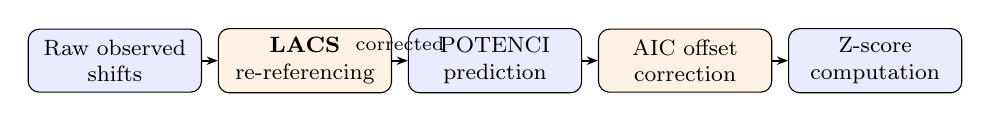
\begin{tikzpicture}[
  box/.style={draw, rounded corners, fill=blue!8, minimum height=0.8cm, minimum width=2.2cm, align=center, font=\footnotesize},
  bigbox/.style={draw, rounded corners, fill=orange!10, minimum height=0.8cm, minimum width=2.2cm, align=center, font=\footnotesize},
  arr/.style={-{Stealth[length=4pt]}, thick},
  node distance=0.2cm
]
  \node[box] (raw) {Raw observed\\shifts};
  \node[bigbox, right=of raw] (lacs) {\textbf{LACS}\\re-referencing};
  \node[box, right=of lacs] (potenci) {POTENCI\\prediction};
  \node[bigbox, right=of potenci] (offset) {AIC offset\\correction};
  \node[box, right=of offset] (zscore) {Z-score\\computation};

  \draw[arr] (raw) -- (lacs);
  \draw[arr] (lacs) -- node[above, font=\scriptsize]{corrected} (potenci);
  \draw[arr] (potenci) -- (offset);
  \draw[arr] (offset) -- (zscore);
\end{tikzpicture}
\end{center}

\medskip
\textbf{Two complementary systems:}
\begin{enumerate}\setlength\itemsep{2pt}
  \item \textbf{LACS} (before POTENCI): Wishart 1995 random coil tables. Works on all residues.
  \item \textbf{POTENCI-based offset} (after): POTENCI predictions + AIC model selection + 9-residue rolling window.
\end{enumerate}

\medskip
\textbf{Status:} LACS module complete \& validated against 6,774 BMRB LACS reports.\\
Integration into scoring pipeline in progress.
\end{frame}

% ═══════════════════════════════════════════════════════════════════
% SLIDE: Limitations
% ═══════════════════════════════════════════════════════════════════
\begin{frame}{Limitations}

\begin{itemize}\setlength\itemsep{4pt}
  \item \textbf{Requires secondary shift spread.} IDPs with near-zero secondary shifts $\Rightarrow$ poorly determined regression. Less relevant for TriZOD (most BMRB entries are structured).

  \item \textbf{CA and CB offsets are coupled.} Both share the ${}^{13}$C reference $\Rightarrow$ always near-identical offsets. Cannot detect atom-type-specific errors.

  \item \textbf{HB is inferred, not measured.} No direct LACS relationship for HB; offset propagated from HA.

  \item \textbf{Assumes constant offset.} Single constant per nucleus type. Position-dependent errors (rare) are not detected.
\end{itemize}
\end{frame}

% ═══════════════════════════════════════════════════════════════════
% SLIDE: Summary
% ═══════════════════════════════════════════════════════════════════
\begin{frame}{Summary}

\begin{enumerate}
  \item NMR referencing errors are \textbf{common} ($\sim$20\% ${}^{13}$C, $\sim$35\% ${}^{15}$N) and bias downstream analyses.

  \medskip
  \item LACS detects offsets using the \textbf{reference-independent} CA$-$CB difference as X-axis.

  \medskip
  \item Two-line robust regression handles the \textbf{V-shape} from helix/strand residues.

  \medskip
  \item The \textbf{Y-intercept} directly gives the referencing error (sign: positive $=$ too high).

  \medskip
  \item Our Python reimplementation validates against BMRB LACS reports and serves as the first correction step in the TriZOD pipeline.
\end{enumerate}
\end{frame}

\end{document}
